\documentclass[12pt, a4paper]{article}

%% abstract (?)
\usepackage{authblk}
\usepackage[top=2cm, bottom=2cm, left=2cm, right=2cm]{geometry}
\usepackage{fancyhdr}
%% abstract (?)

\usepackage{amssymb}
\usepackage{amsthm}
\usepackage{amscd}
\usepackage{amsmath}
\usepackage{enumitem}

\usepackage{multicol, fullpage}

\usepackage{esint} %Lines up double+ integrals
\usepackage[usenames,dvipsnames]{xcolor} % allows you to use color names, call this BEFORE you call TikZ
\usepackage{tikz, tikz-3dplot, pgfplots}
\usepackage{tkz-graph}
\usepackage{tensor}

\usepackage{graphicx}
\usepackage{caption}
\usepackage{subcaption}
\usepackage{cancel}



\usetikzlibrary{hobby}
\pgfplotsset{compat=1.8}


\usetikzlibrary{calc}


\setlength{\evensidemargin}{1in}
\addtolength{\evensidemargin}{-1in}
\setlength{\oddsidemargin}{1.5in}
\addtolength{\oddsidemargin}{-1.5in}
\setlength{\topmargin}{1in}
\addtolength{\topmargin}{-1.5in}

\setlength{\textwidth}{16cm}
\setlength{\textheight}{23cm}


\theoremstyle{plain}
\newtheorem{theorem}{Theorem}[section]
\newtheorem{lemma}{Lemma}
\newtheorem{proposition}{Proposition}
\newtheorem*{corollary}{Corollary}


\theoremstyle{definition}
\newtheorem{definition}{Definition}[section]
\newtheorem{notation}{Notation}
\newtheorem{question}{Question}
\newtheorem{conjecture}{Conjecture}[section]
\newtheorem{solution}{Solution}[section]
\newtheorem{example}{Example}[section]
\newtheorem{counter}{Counter Example}[section]


\theoremstyle{remark}
\newtheorem*{rem}{Remark}
\newtheorem*{note}{Note}


\def\proof{\noindent {\it Proof.} \hskip 0.1in}
\def\qed{\rightline{$\blacklozenge$}}

\newcommand{\RR}{\mathbb{R}}
\newcommand{\QQ}{\mathbb{Q}}
\newcommand{\NN}{\mathbb{N}}
\newcommand{\ZZ}{\mathbb{Z}}
\newcommand{\CC}{\mathbb{C}}
\newcommand{\II}{\mathbb{I}}

%unnecessary?
%\pagestyle{fancy}



\renewenvironment{abstract}{%
\hfill\begin{minipage}{0.95\textwidth}
\rule{\textwidth}{1pt}}
{\par\noindent\rule{\textwidth}{1pt}\end{minipage}}
%
\makeatletter
\renewcommand\@maketitle{%
\hfill
\begin{minipage}{0.95\textwidth}
\vskip 2em
\let\footnote\thanks 
{\LARGE \@title \par }
\vskip 1.5em
{\large \@author \par}
\end{minipage}
\vskip 1em \par
}
\makeatother
%
\begin{document}
%
%title and author details
\title{Cardiovascular Flow in Cylindrical Domain}
\author{Sean Kearns, Victor Ruiz}
%
\maketitle
%
\begin{abstract}
This project will briefly introduce the study of cardiovascular fluids, and discuss current analytical and numerical solutions. Assuming Newtonian flow will inherently limit this discussion to larger vessels, but will allow for a simpler problem construction using the Navier-Stokes equations. %The incompressibility, steady flow, laminar, and ??
\end{abstract}
\section{Introduction}
Cardiovascular disease (CVD) claims over 17 million lives every year, thus very quickly becoming one of the leading causes of death around the world. The difficulty with such an intricate collection of diseases is that detection is typically invasive and dangerous. Hence, having analytical or numerical blood flow models accurately describing the circulatory system would contribute to the creation of alternative methods of diagnosis, and treatment of CVDs $[3]$.




%theoretical and historical construction (day 1), and physical/reality check (day 2)?

It was not until the 19th century that J.P. Poiseuille produced the first simplified mathematical model of fluid flow in a cylindrical pipe (fluid parcel). Thereafter, contributors such as T. Young (elasticity of arterial tissues and blood pressure propagation), O. Frank (electric network analogy), and J. Womersley (periodic pressure gradients) have been associated with analytical hemodynamical problems $[1]$. A modified version of the incompressible Navier-Stokes equations in axisymmetric coordinates as demonstrated by Nithiarasu will be considered to expose the challenges of analytical solutions to blood flow problems $[4]$. One particular numerical model using CT scans and axial geometry shown by Jane et. al. in $[3]$ will also be considered to express the value of numerical solutions to cardiovascular fluid PDEs.





\begin{figure}[ht!]
\centering
\begin{subfigure}[b]{0.3\textwidth}
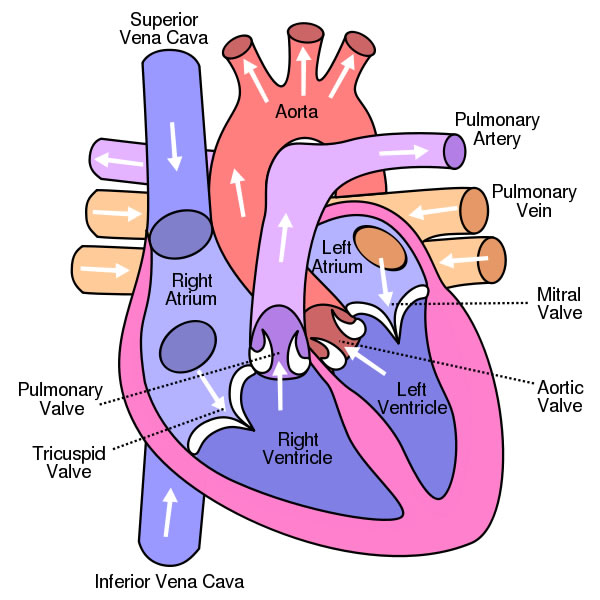
\includegraphics[width=50mm]{HeartDiagram.jpg}
\caption{Heart Diagram}
\end{subfigure}
\begin{subfigure}[b]{0.3\textwidth}
                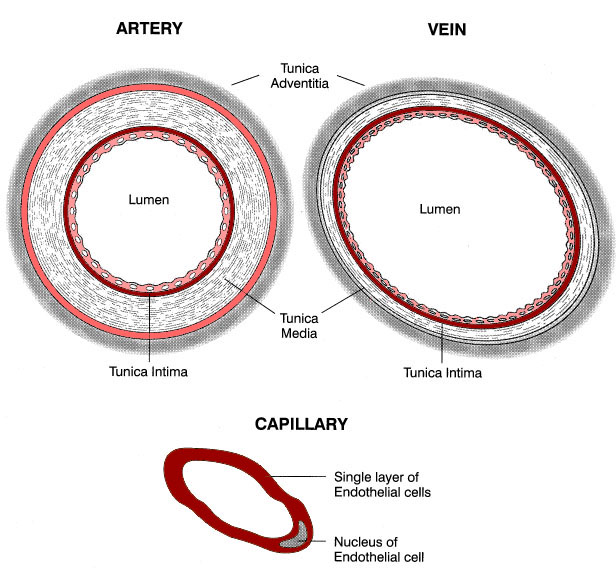
\includegraphics[width=50mm]{ArteryWall.jpg}
                \caption{Artery Wall}
\end{subfigure}
\begin{subfigure}[b]{0.3\textwidth}
                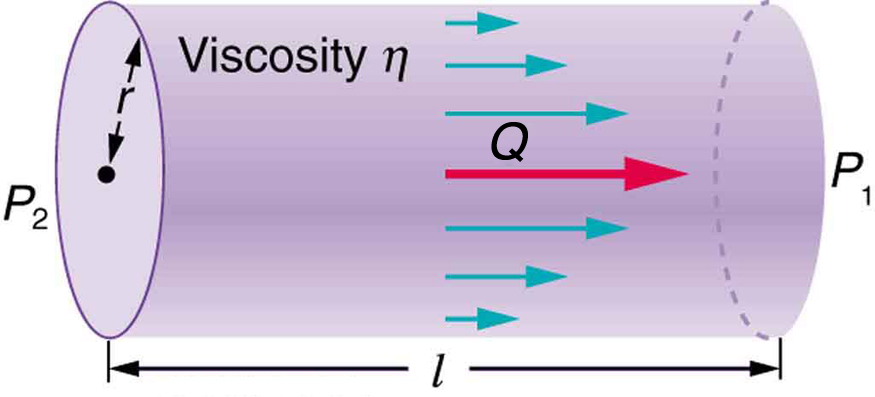
\includegraphics[width=50mm]{ProjectDomain.jpg}
                \caption{Prospective Domain}
\end{subfigure}
\end{figure}

$\vspace{.5in}$

%What do we plan to do in this paper?

%In order to stick to Newtonian fluids we plan to observe blood flow through a large artery (probably the left ventrical) so that the size of the red blood cells with respect to the vessel diameter does not create complicating shears in the chosen domain (vessel--cylinder toy problem?).



\section{Problem Formulation}
%Define variables, and equations in this formulation of the Navier-Stokes equations


Note that this is an analytical construction of a crude blood flow problem $[4]$. Referencing figure 2, the incompressible Navier-Stokes equations in axisymmetric coordinates, can be written as 
\begin{align}
\frac{1}{r}\frac{\partial}{\partial r} (ru_r) + \frac{\partial u_z}{\partial z} = 0 \\
\frac{\partial u_r}{\partial t} + u_r \frac{\partial u_r}{\partial r} + u_z \frac{\partial u_r}{\partial z} = -\frac{1}{\rho} \frac{\partial p}{\partial x} + \nu \left[  \frac{\partial}{\partial r} \left( \frac{1}{r} \frac{\partial}{\partial r} (ru_r)  \right) + \frac{\partial^2u_r}{\partial z^2}       \right]\\
\alpha^2\frac{\partial u_z}{\partial t} + u_r \frac{\partial u_z}{\partial r} + u_z \frac{\partial u_z}{\partial z} = -\frac{1}{\rho} \frac{\partial p}{\partial z} + \nu \left[  \frac{\partial}{\partial r} \left( \frac{1}{r} \frac{\partial}{\partial r} (ru_z)  \right) + \frac{\partial^2u_z}{\partial z^2}       \right]
\end{align}
where the circumferential velocity is assumed to be zero (i.e. $u_{\phi} = 0$). 

\begin{figure}[ht!]
\centering
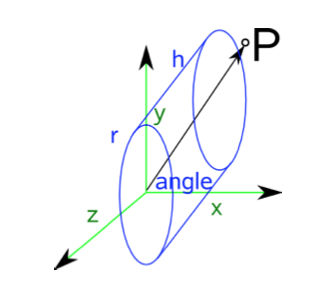
\includegraphics[width=50mm]{cylindricalcoordinates.png}
\caption{Cylindrical coordinates}
\end{figure}



Supposing that the fluid in question is Newtonian, then any derivative $\frac{\partial u}{\partial z}$ or $u_r$ will also be zero.

%what does it mean to be a newtonian fluid?
%what does it mean for the fluid itself to assume circumferential velocity, z axial derivatives, and radial velocity are zero?



%Fluid assumptions4

As such, the Navier-Stokes equations are reduced as follows:
\begin{align}
\frac{1}{r}\frac{\partial}{\partial r} (r\cancelto{0}{u_r}) + \cancelto{0}{\frac{\partial u_z}{\partial z}} = 0 \\
\cancelto{0}{\frac{\partial u_r}{\partial t}} + \frac{\partial u_r}{\partial r}\cancelto{0}{u_r} + u_z \cancelto{0}{\frac{\partial u_r}{\partial z}} = -\frac{1}{\rho} \frac{\partial p}{\partial x} + \nu \left[  \frac{\partial}{\partial r} \left( \frac{1}{r} \frac{\partial}{\partial r} (r\cancelto{0}{u_r})  \right) + \cancelto{0}{\frac{\partial^2u_r}{\partial z^2}}       \right]\\
\alpha^2\frac{\partial u_z}{\partial t} + \frac{\partial u_z}{\partial r}\cancelto{0}{u_r} + u_z \cancelto{0}{\frac{\partial u_z}{\partial z}} = -\frac{1}{\rho} \frac{\partial p}{\partial z} + \nu \left[  \frac{\partial}{\partial r} \left( \frac{1}{r} \frac{\partial}{\partial r} (ru_z)  \right) + \cancelto{0}{\frac{\partial^2u_z}{\partial z^2}}       \right]
\end{align}

Thus, equations 4,5, and 6 are reduced to 
\begin{align}
 \alpha^2\frac{\partial u_z}{\partial t} = -\frac{1}{\rho} \frac{\partial p}{\partial z} + \frac{\nu}{r} \frac{\partial}{\partial r} \left(  r \frac{\partial u_z}{\partial r}   \right)
\end{align}
assuming that the pressure gradient in the $x$-direction remains zero, and where $\alpha=R\sqrt{\frac{\omega}{\nu}}$ is the Womersley number). If focusing on vessels such as veins, or arterioles and capillaries with a very low Womersley number ($\alpha < < 1$), then the first term in ($7$) goes to zero.

\begin{align}
 \cancelto{0}{\alpha^2\frac{\partial u_z}{\partial t}} = -\frac{1}{\rho} \frac{\partial p}{\partial z} + \frac{\nu}{r} \frac{\partial}{\partial r} \left(  r \frac{\partial u_z}{\partial r}   \right)
\end{align}

Given $\nu = \mu / \rho$ as the dynamic viscocity, then equation $(8)$ becomes (assuming blood density $\rho=1$--equivalent to water)

\begin{align}
 \frac{1}{\rho} \frac{\partial p}{\partial z} = \frac{\nu}{r} \frac{\partial}{\partial r} \left(  r \frac{\partial u_z}{\partial r}   \right)\\
\frac{r}{\mu} \frac{\partial p}{\partial z} = \frac{\partial}{\partial r} \left(  r \frac{\partial u_z}{\partial r}   \right)
\end{align}

In order to solve for $u_z$ and eventually the flow rate $Q$ we shall integrate equation $(10)$ twice with respect to $r$. Note that pressure $p$ isn't a function of $r$. Also, integrating twice we will generate a linear term as well as a constant term which will be added on at the end. %ask gustafson is this is possible to do as in the book, seems sketchy or unreasonable in some way

\begin{align}
\frac{r}{\mu} \frac{\partial p}{\partial z} &= \frac{\partial}{\partial r} \left(  r \frac{\partial u_z}{\partial r}   \right) \\
\int \frac{r}{\mu} \frac{\partial p}{\partial z} \, dr &= \int \frac{\partial}{\partial r} \left(  r \frac{\partial u_z}{\partial r}   \right) \, dr \\
\frac{r^2}{2\mu} \frac{\partial p}{\partial z} &= r \frac{\partial u_z}{\partial r} \\
\frac{r}{2\mu} \frac{\partial p}{\partial z} &= \frac{\partial u_z}{\partial r} \\
\int \frac{r}{2\mu} \frac{\partial p}{\partial z} \, dr &= \int \frac{\partial u_z}{\partial r} \, dr \\
\frac{r^2}{4\mu} \frac{\partial p}{\partial z} &= u_z 
\end{align}
Introducing the linear and constant terms generated from the constants of integration, we have
\begin{align}
u_z  = \frac{r^2}{4\mu} \frac{\partial p}{\partial z} + ar + b 
\end{align}

Note that we add on the linear and constant terms at the end to avoid a blow-up term. Now, to solve for constants $a$ and $b$, the chosen boundary conditions must be applied before calculating the flow rate $Q$ through a slice of the cylinder.


With the assumptions that $\partial u_z/\partial r = 0$ at $r=0$ and $r=R$, $u_z=0$ we find that $a=0$ and $b= - \frac{R^2}{4\mu} \frac{\partial p }{\partial z}$.
 
$\vspace{.05in}$
To find $a$,
\begin{align}
u_z  &= \frac{r^2}{4\mu} \frac{\partial p}{\partial z} + ar + b  \\
0 = \partial u_z/\partial r &= \underbrace{\frac{r}{2\mu} \frac{\partial p}{\partial z}} + a \\
&\text{at $r=0$} \rightarrow a=0 
\end{align}

To find $b$, 
\begin{align}
0 = u_z  &= \frac{R^2}{4\mu} \frac{\partial p}{\partial z} + 0 \cdot r + b  \\
b &=  - \frac{R^2}{4\mu} \frac{\partial p}{\partial z}
\end{align}

After substituting $a$ and $b$ back into $u_z$ we obtain
\begin{align}
u_z  &= \frac{r^2}{4\mu} \frac{\partial p}{\partial z} + ar + b  \\
u_z  &= \frac{r^2}{4\mu} \frac{\partial p}{\partial z} - \frac{R^2}{4\mu} \frac{\partial p}{\partial z}  \\
u_z  &= - \frac{R^2}{4\mu} \frac{\partial p}{\partial z} \left[    1-\frac{r^2}{R^2}      \right]
\end{align}

To find the flow rate $Q$ through a cross-section of the cylinder (circle of radius $R$) in Figure $2$, we have 

\begin{align}
u_z  &= - \frac{R^2}{4\mu} \frac{\partial p}{\partial z} \left[    1-\frac{r^2}{R^2}      \right] \\
\text{why this is the flux?} \quad \rightarrow \; Q &= \int_0^{2\pi}\int_0^R \frac{r^2}{4\mu} \frac{\partial p}{\partial z} - \frac{R^2}{4\mu} \frac{\partial p}{\partial z} \, rdrd\theta \\
 &= \int_0^{2\pi}\int_0^R \frac{r^3}{4\mu} \frac{\partial p}{\partial z} - \frac{R^2r}{4\mu} \frac{\partial p}{\partial z} \, drd\theta \\
 &= \int_0^{2\pi} \frac{r^4}{16\mu} \frac{\partial p}{\partial z} - \frac{R^2r^2}{8\mu} \frac{\partial p}{\partial z} \, \Big|_0^R d\theta \\
 &= \int_0^{2\pi} \frac{R^4}{16\mu} \frac{\partial p}{\partial z} - \frac{R^4}{8\mu} \frac{\partial p}{\partial z} \, d\theta \\
 &= \frac{\theta R^4}{16\mu} \frac{\partial p}{\partial z} - \frac{\theta R^4}{8\mu} \frac{\partial p}{\partial z} \, \Big|_0^{2\pi} \\
 &= \frac{2\pi R^4}{16\mu} \frac{\partial p}{\partial z} - \frac{2\pi R^4}{8\mu} \frac{\partial p}{\partial z} \\
Q &= - \frac{\pi R^4}{8\mu} \frac{\partial p}{\partial z} 
\end{align}
% rigid tube, newtonian flow, steady --> simplest case (quickly derive and explain assumptions made, and how they correspond to the actual problem/domain)

% Neglect the newtonian flow assumption for a moment, and show the equations in comparison to newtonian flow --> perfect segway using quote in "Biofluids" [43] explaining how crude of an approximation this is, even after oversimplifying the problem, AND the domain.

% --> Brief introduction to the paper presenting a numerical model of a vessel splitting
% End












\newpage


 \begin{thebibliography}{1}
 \bibitem{history} Alfio Quarteroni, {\em Modeling the Cardiovascular System--A Mathematical Adventure: Part I.} 2001: SIAM News 34.5 (2001): 1-3.

  \bibitem{n-seq} C Y Wang, {\em Exact solutions of the unsteady Navier-Stokes equations.} 1989: American Society of Mechanical Engineers.

  \bibitem{carotid}  Jhalique Jane R. Fojas, Rizalinda L. De Leon, {\em Carotid Artery Modeling Using the Navier-Stokes Equations for an Incompressible, Newtonian and Axisymmetric Flow.} 2013: Asia-Pacific Chemical, Biological $\&$ Environmental Engineering Society.


  \bibitem{Biofluid} Perumal Nithiarasu {\em Biofluid Dynamics.} 2008: Swansea University, United Kingdom.

  \bibitem{Newtonian Fluid} Suares Clovis Oukouomi Noutchie, {\em Flow of a Newtonian Fluid: The Case of Blood in Large Arteries.} 2005 (Unpublished (?) masters dissertation): University of South Africa, South Africa.

  \end{thebibliography}

\end{document}